\documentclass[handout]{beamer}

%\usepackage{movie15}

\usepackage{tikz}
\usetikzlibrary{shapes, arrows, calc}

\usepackage[T1]{fontenc}
\usepackage[ansinew]{inputenc}
\usepackage{lmodern} 
\usepackage{textcomp}

\useoutertheme{infolines} 
\setbeamertemplate{navigation symbols}{}
\setbeamertemplate{items}[ball] 
\setbeamertemplate{blocks}[rounded][shadow=true] 

%\usetheme{Boadilla}
\usetheme{Madrid}
\usecolortheme{whale}

\author[Boshen Chen]{Boshen Chen \\{\small Supervised by: Dr.\ Andrea Raith, Olga Perederieieva}}

\title[Faster Shortest Path Computation]{Faster Shortest Path Computation for Traffic Assignment}

%\subtitle[]{}

\institute[UoA]{
    Department of Engineering Science\\
    University of Auckland\\
}

\begin{document}

\begin{frame}[plain]
    \titlepage
\end{frame}

\begin{frame}{Contents}
    \tableofcontents
\end{frame}

\section{Project motivation - Traffic Assignment}
\begin{frame}{Transportation forecasting}

    \begin{columns}
        \begin{column}{0.5\paperwidth}
            \begin{center}
                \tikzstyle{block} = [rectangle, draw, text width=10em, text centered, rounded corners, minimum height=2em]
                \tikzstyle{line} = [draw, -latex']
                \begin{tikzpicture}[node distance=4em]
                    \pause

                    \node [block] (first) {Trip Generation};
                    \pause

                    \node [block, below of=first] (second) {Trip Distribution};
                    \path [line] (first) -- (second);
                    \pause

                    \node [block, below of=second] (third) {Mode Choice};
                    \path [line] (second) -- (third);
                    \pause

                    \node [block, below of=third] (fourth) {Traffic Assignment};
                    \path [line] (third) -- (fourth);
                    \pause

                    \path [line] (fourth.west) -- ($(fourth.west)-(0.8,0)$) -- ($(first.west)-(0.8,0)$) -- (first.west);
                    \path [line] ($(second.west)-(0.8,0)$) -- (second.west);
                    \path [line] ($(third.west)-(0.8,0)$) -- (third.west);
                \end{tikzpicture}
            \end{center}
        \end{column}

        %\begin{column}{0.5\paperwidth}
        %    What has been done in the past \ldots
    % mo%tivation, transportation forecasting and the 4 stage modelling process
    % us%e figure
        %    \begin{itemize}
        %        \item trip generation
        %        \item trip distribution
        %        \item mode choice
        %        \item traffic assignment
        %    \end{itemize}

        %    Traffic assignment
        %    \begin{itemize}
        %        \item how its solved
        %        \item concept of user equilibrium
        %        \item shortest path calculations
        %        \item link cost, lots of iterations, each iteration lots of shortest path calculations
        %    \end{itemize}
        %\end{column}
    \end{columns}

\end{frame}

\section{Solving the Traffic Assignment problem - faster shortest path calculations}
\begin{frame}{Faster shortest path calculations}

    What exist and what I have done \ldots
    \begin{itemize}
        \item Bellman Ford - label correcting algorithm
        \item Dijkstra - label setting algorithm
            \begin{itemize}
                \item different data structures - Heap trees and their advantages
            \end{itemize}
        \item bidirectional
        \item A* search
        \item bidirectional A* search
        \item preprocessing
    \end{itemize}

\end{frame}

\foreach \n in {1,...,7}{
\begin{frame}[shrink]{Dijkstra's Algorithm}
    \begin{center}
        \includegraphics[page=\n,width=\paperwidth, height=\paperheight, keepaspectratio,trim=0 120px 48px 120px,clip]{img/chicago_dijkstra_animation}
    \end{center}
\end{frame}
}

%\begin{frame}[shrink]{Dijkstra's Algorithm}
%    \begin{center}
%        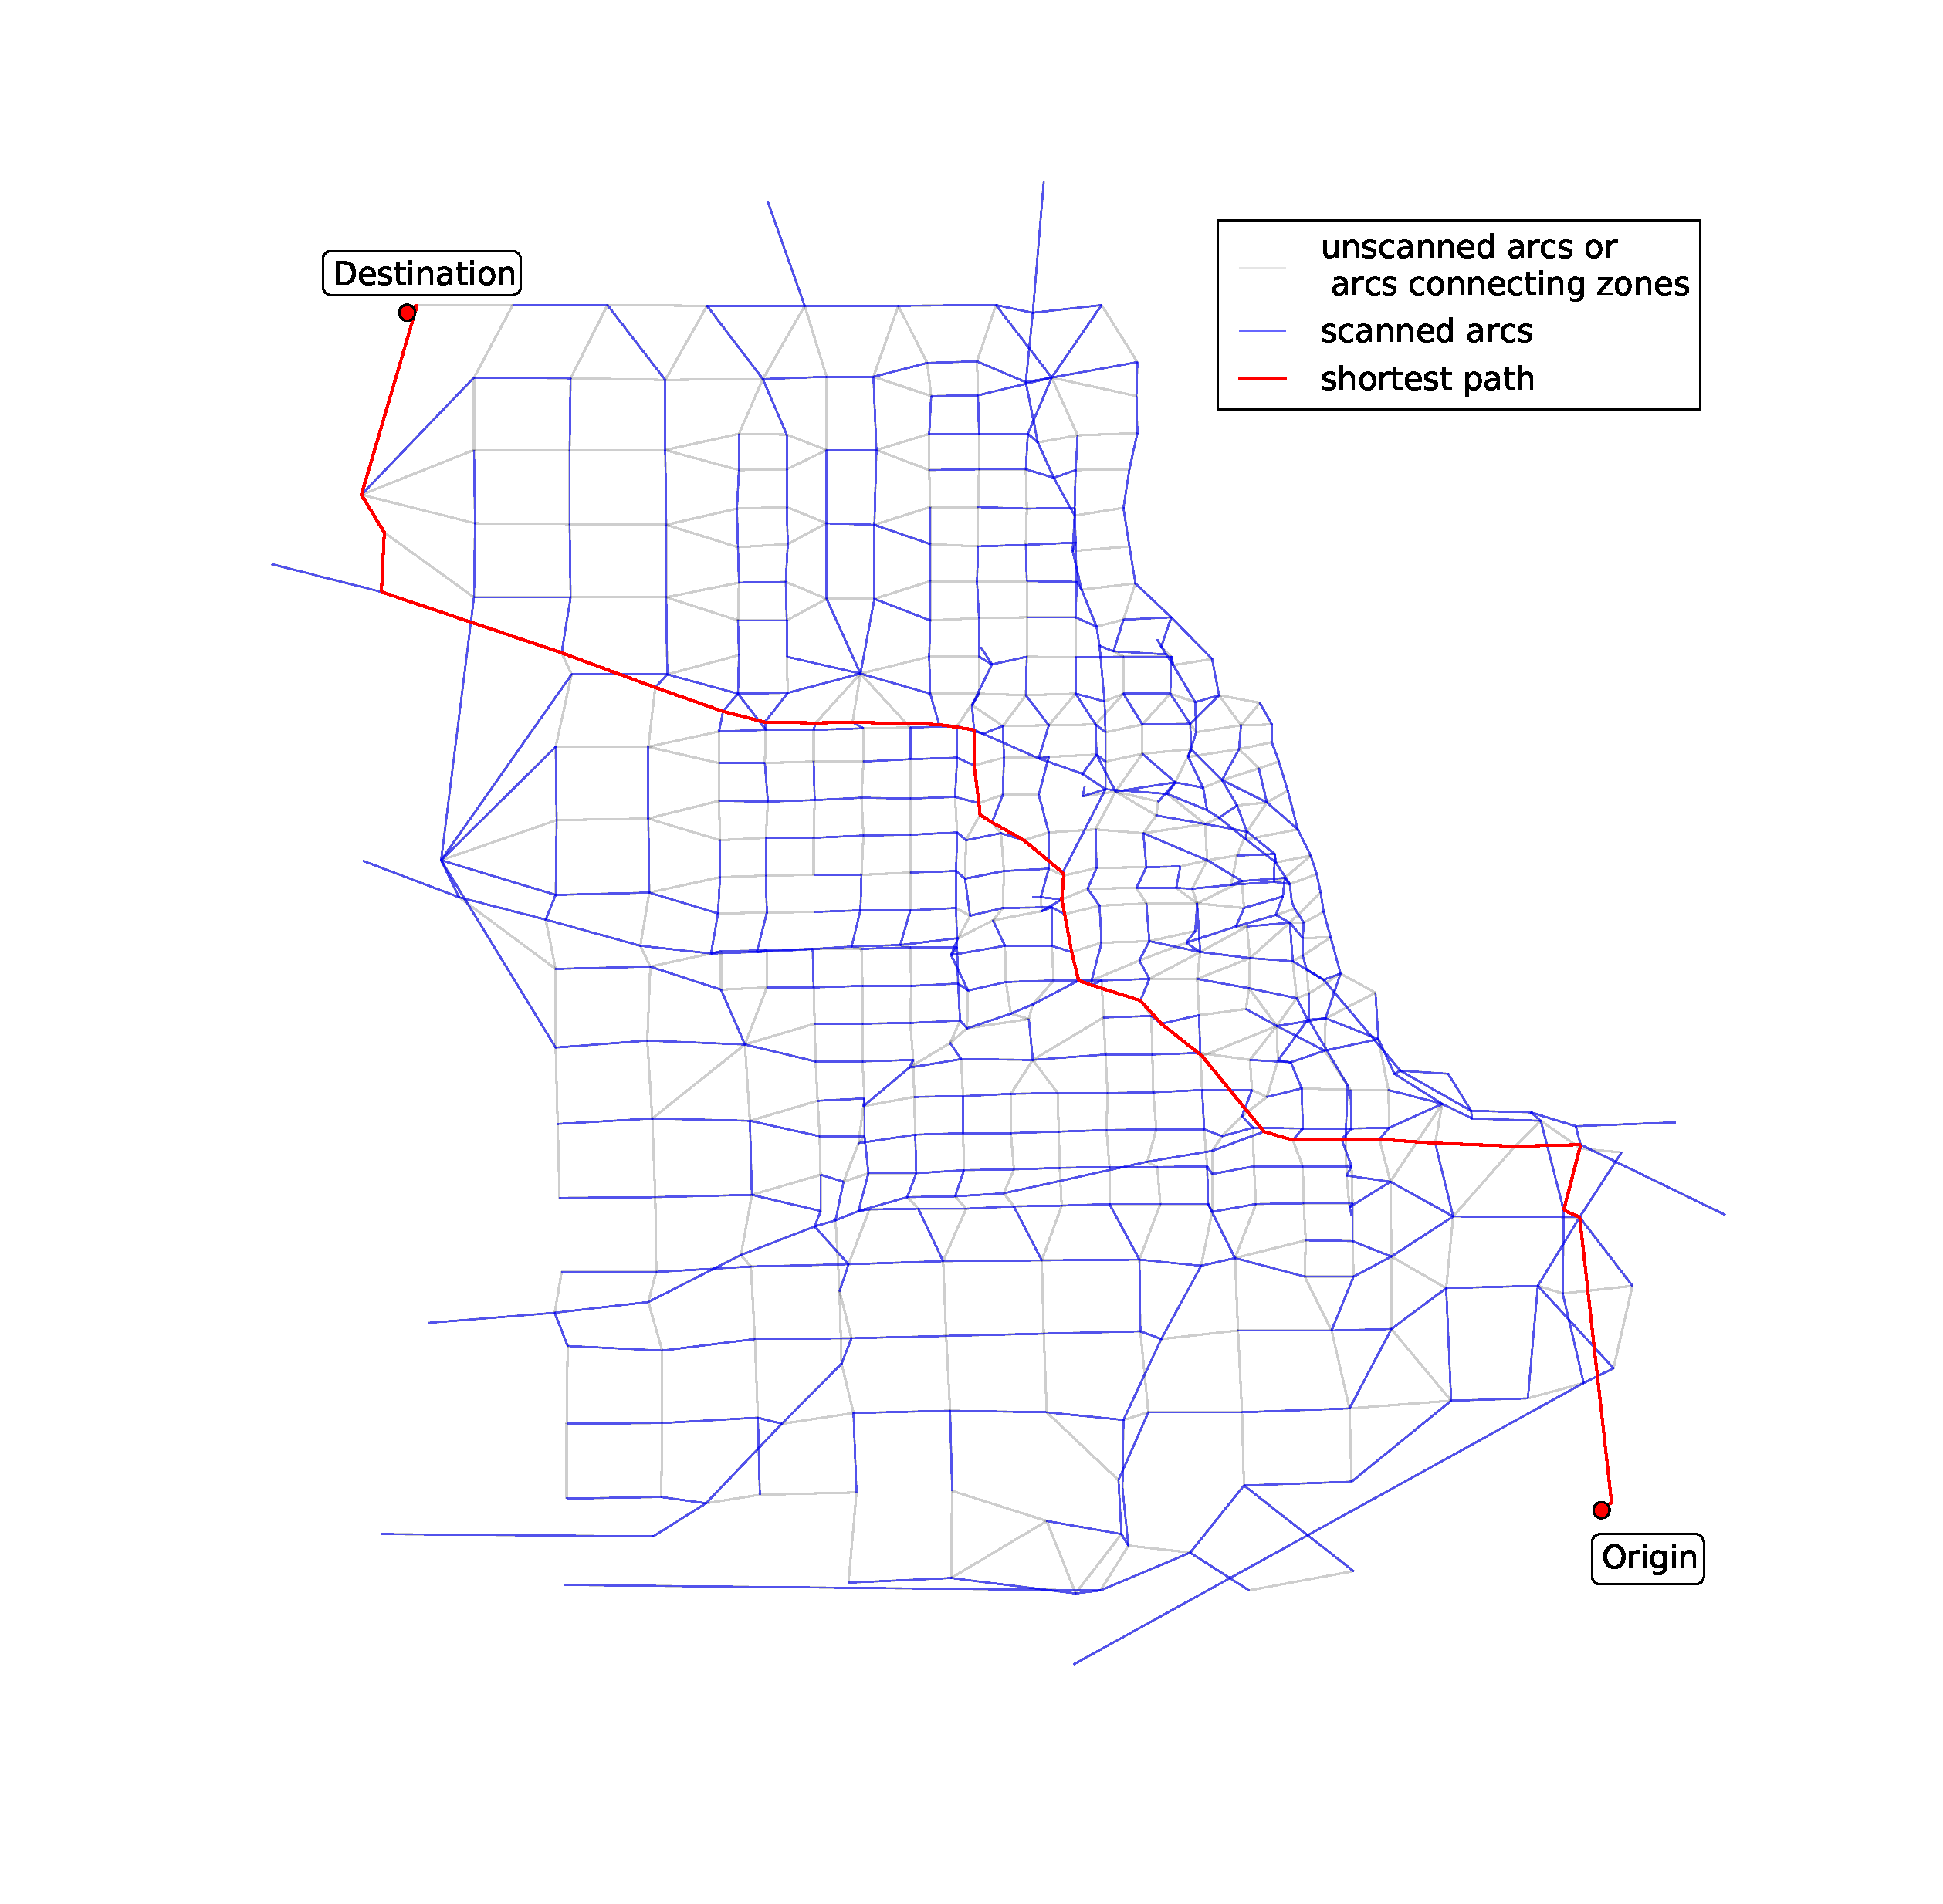
\includegraphics[width=\paperwidth, height=\paperheight, keepaspectratio,trim=0 120px 48px 120px,clip]{img/chicago_dijkstra}
%    \end{center}
%\end{frame}

\begin{frame}[shrink]{Bidirectional Dijkstra's Algorithm}
    \begin{center}
        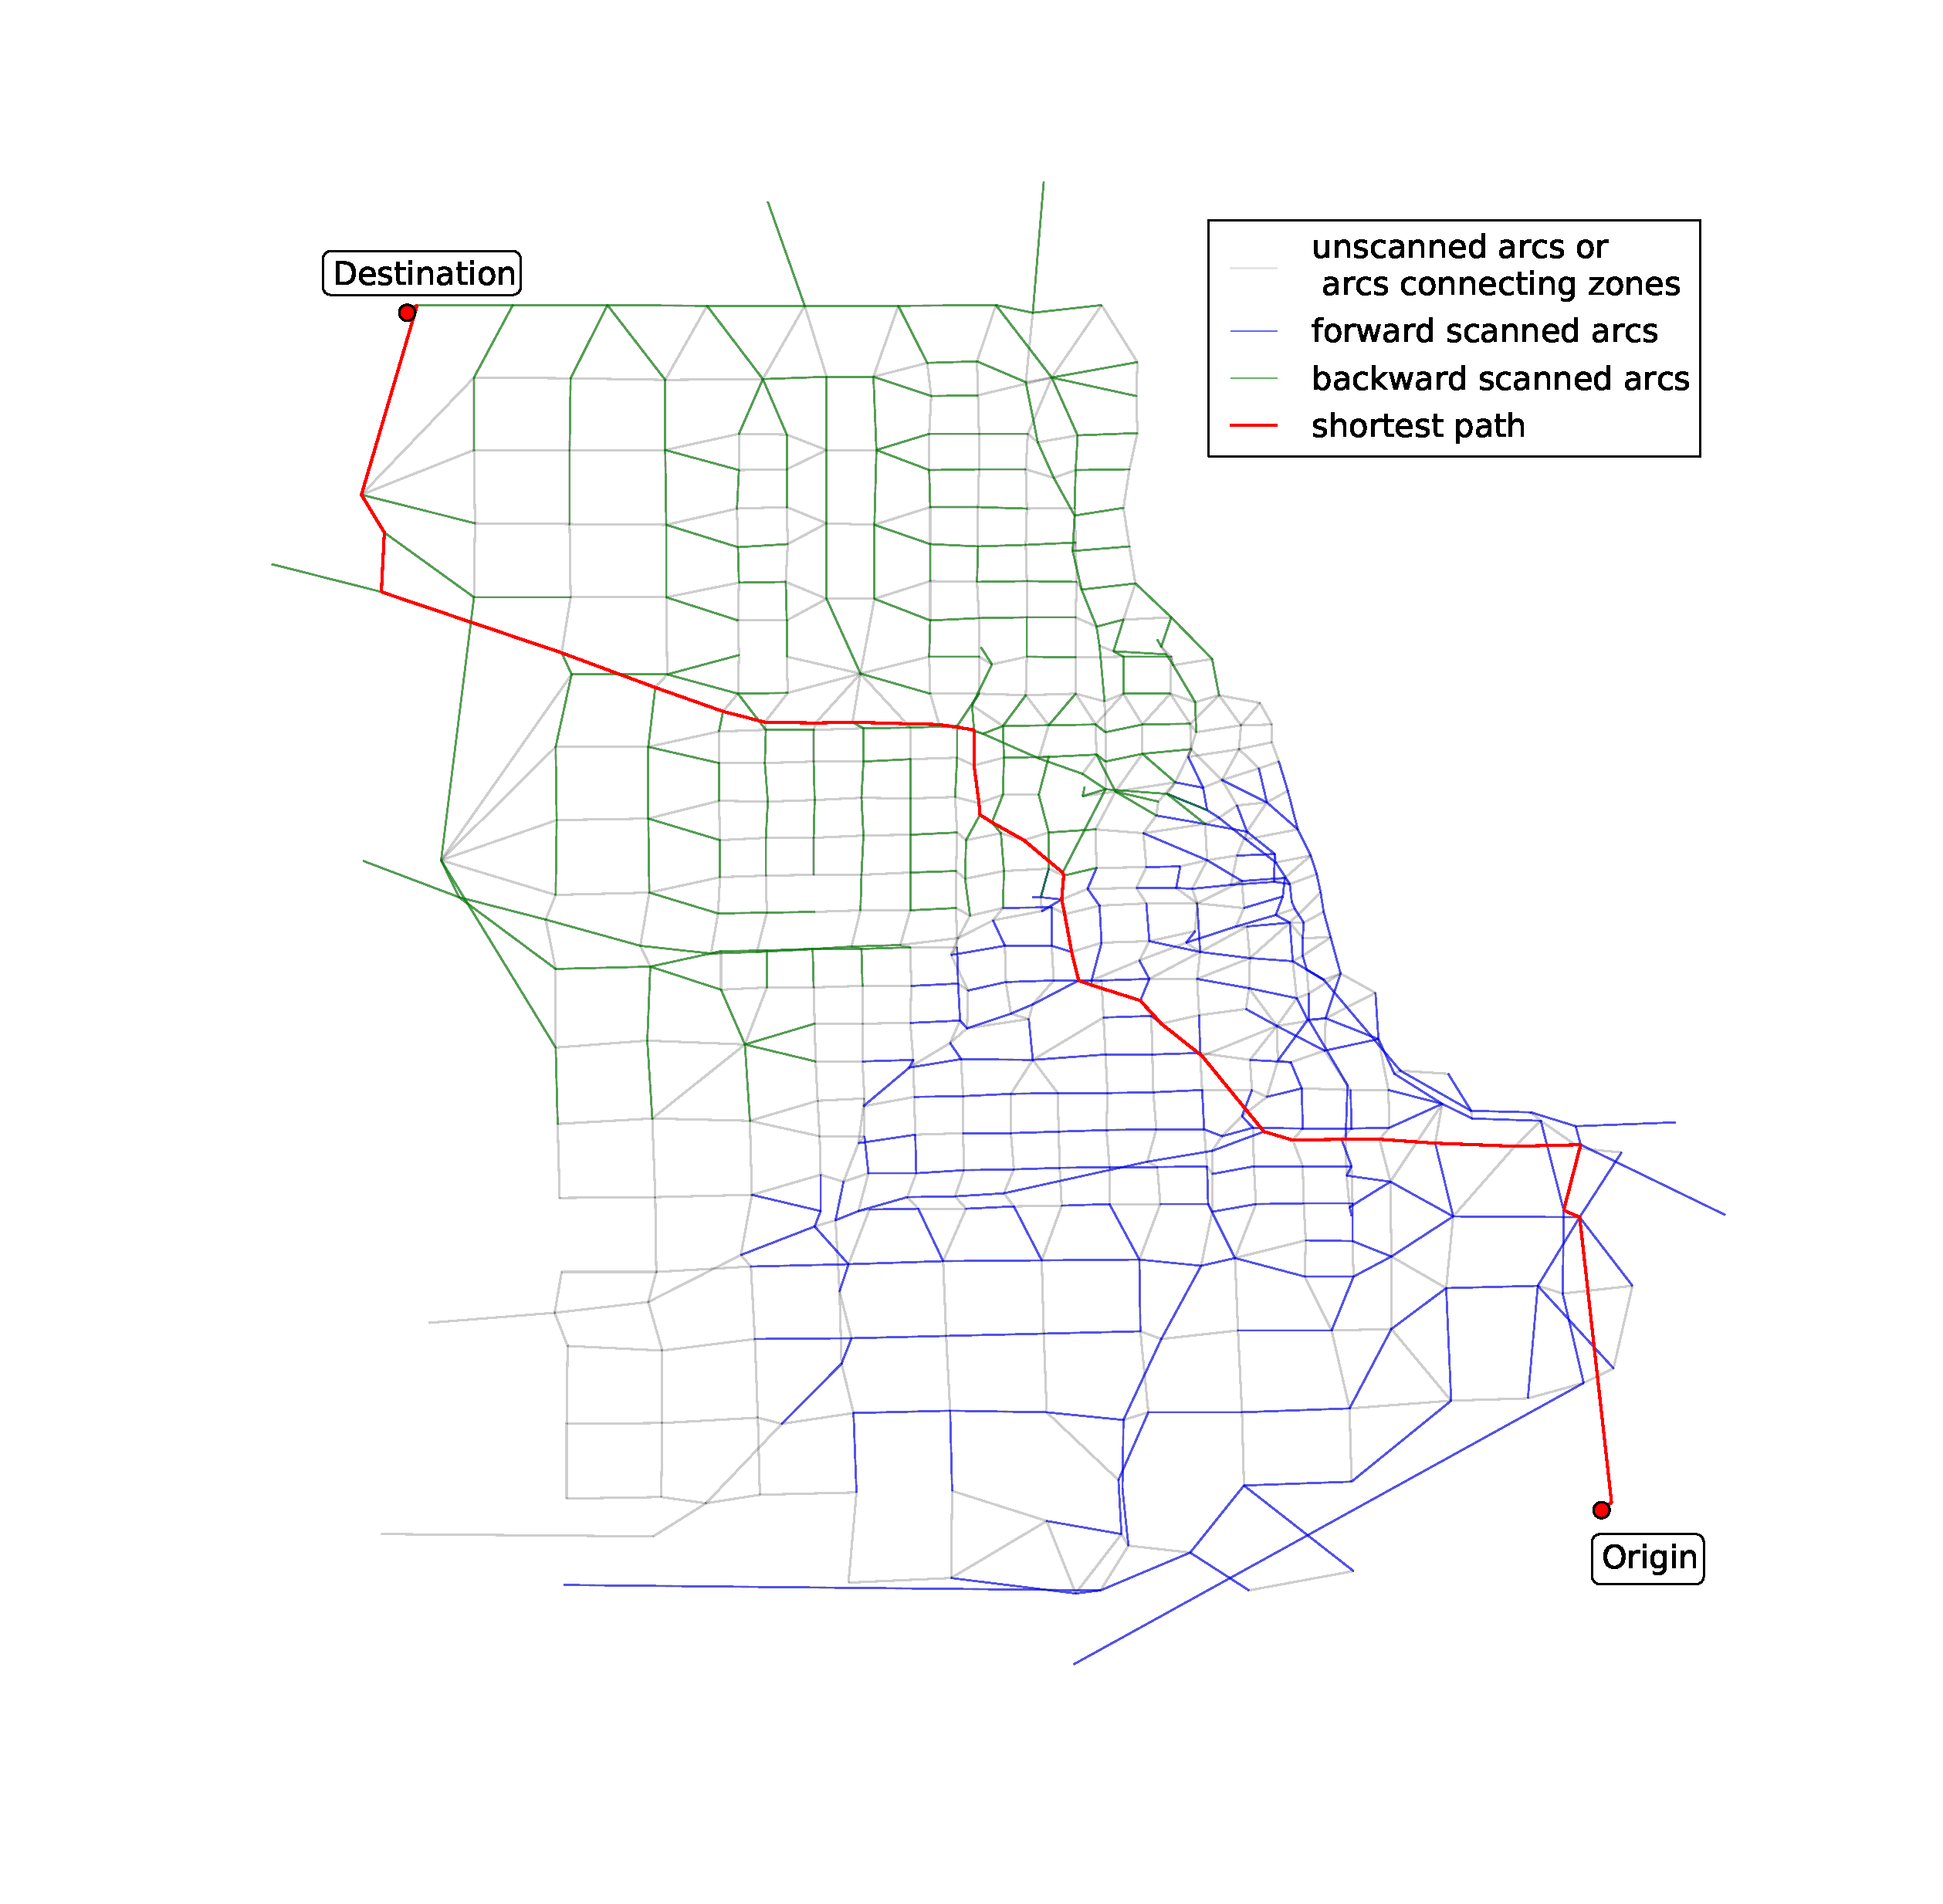
\includegraphics[width=\paperwidth, height=\paperheight, keepaspectratio,trim=0 120px 48px 120px,clip]{img/chicago_bidirect}
    \end{center}
\end{frame}

\begin{frame}[shrink]{A* Search}
    \begin{center}
        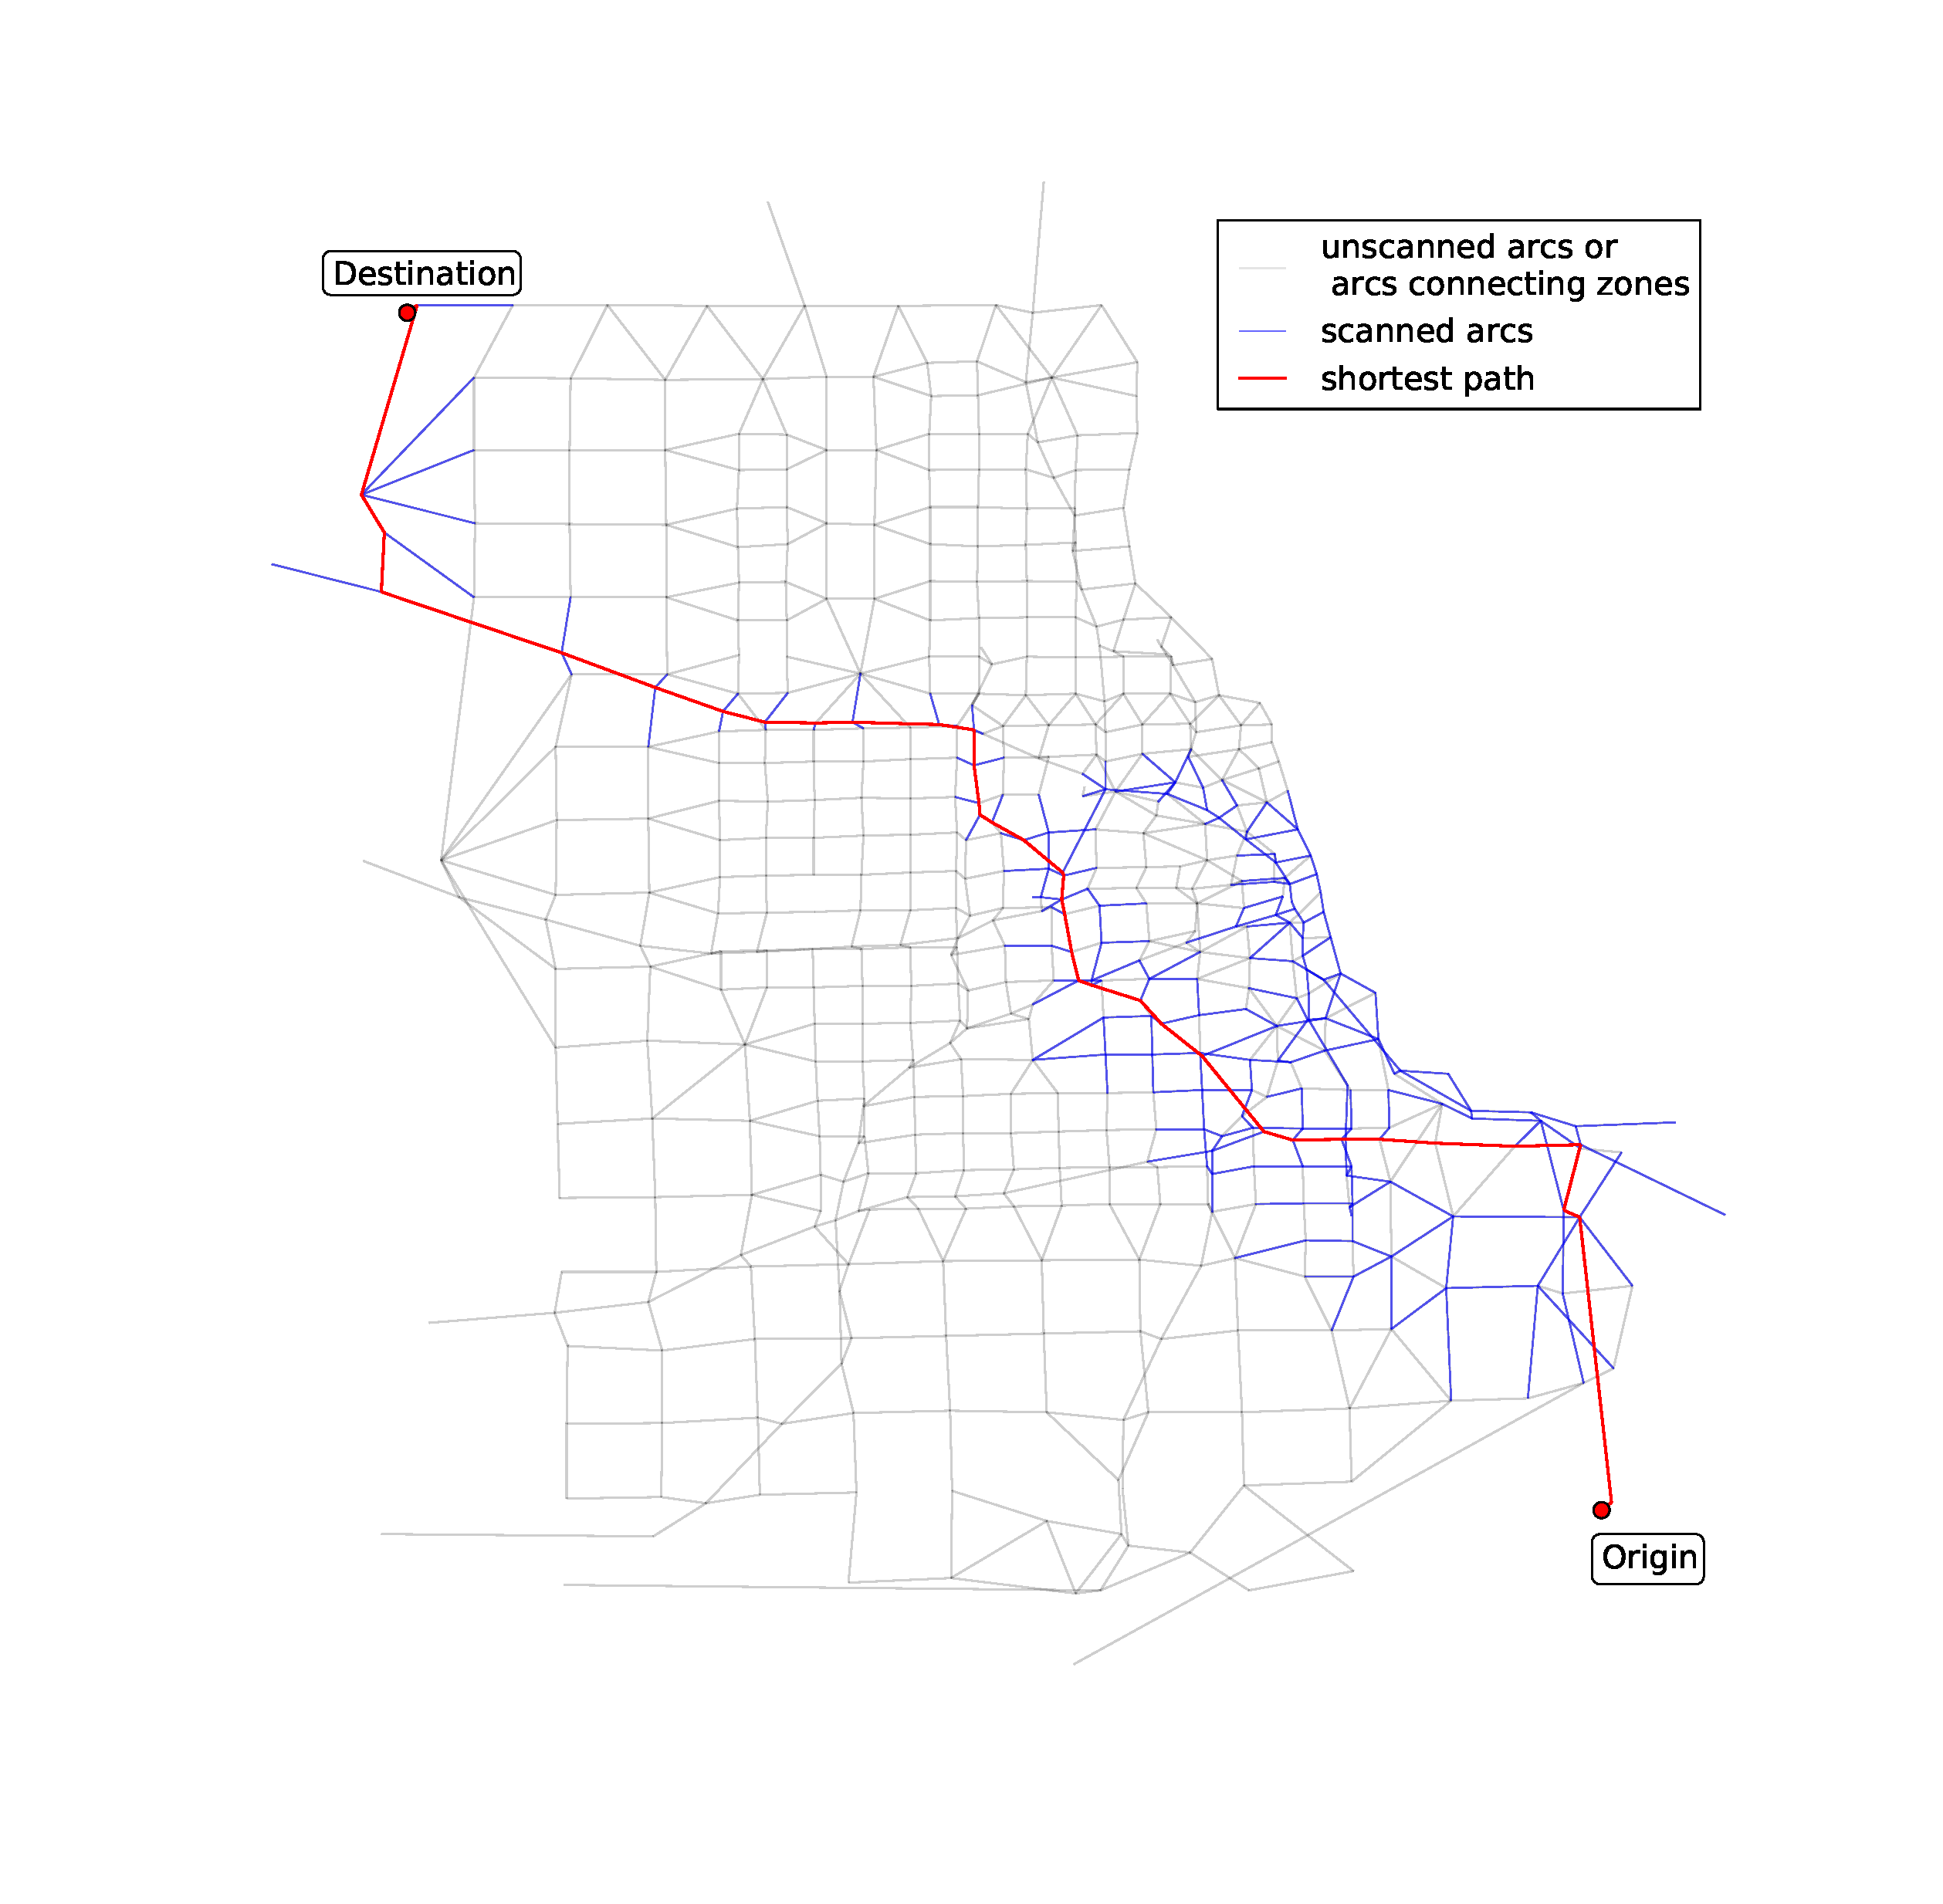
\includegraphics[width=\paperwidth, height=\paperheight, keepaspectratio,trim=0 120px 48px 120px,clip]{img/chicago_astar}
    \end{center}
\end{frame}

\begin{frame}[shrink]{Bidirectional A* Search}
    \begin{center}
        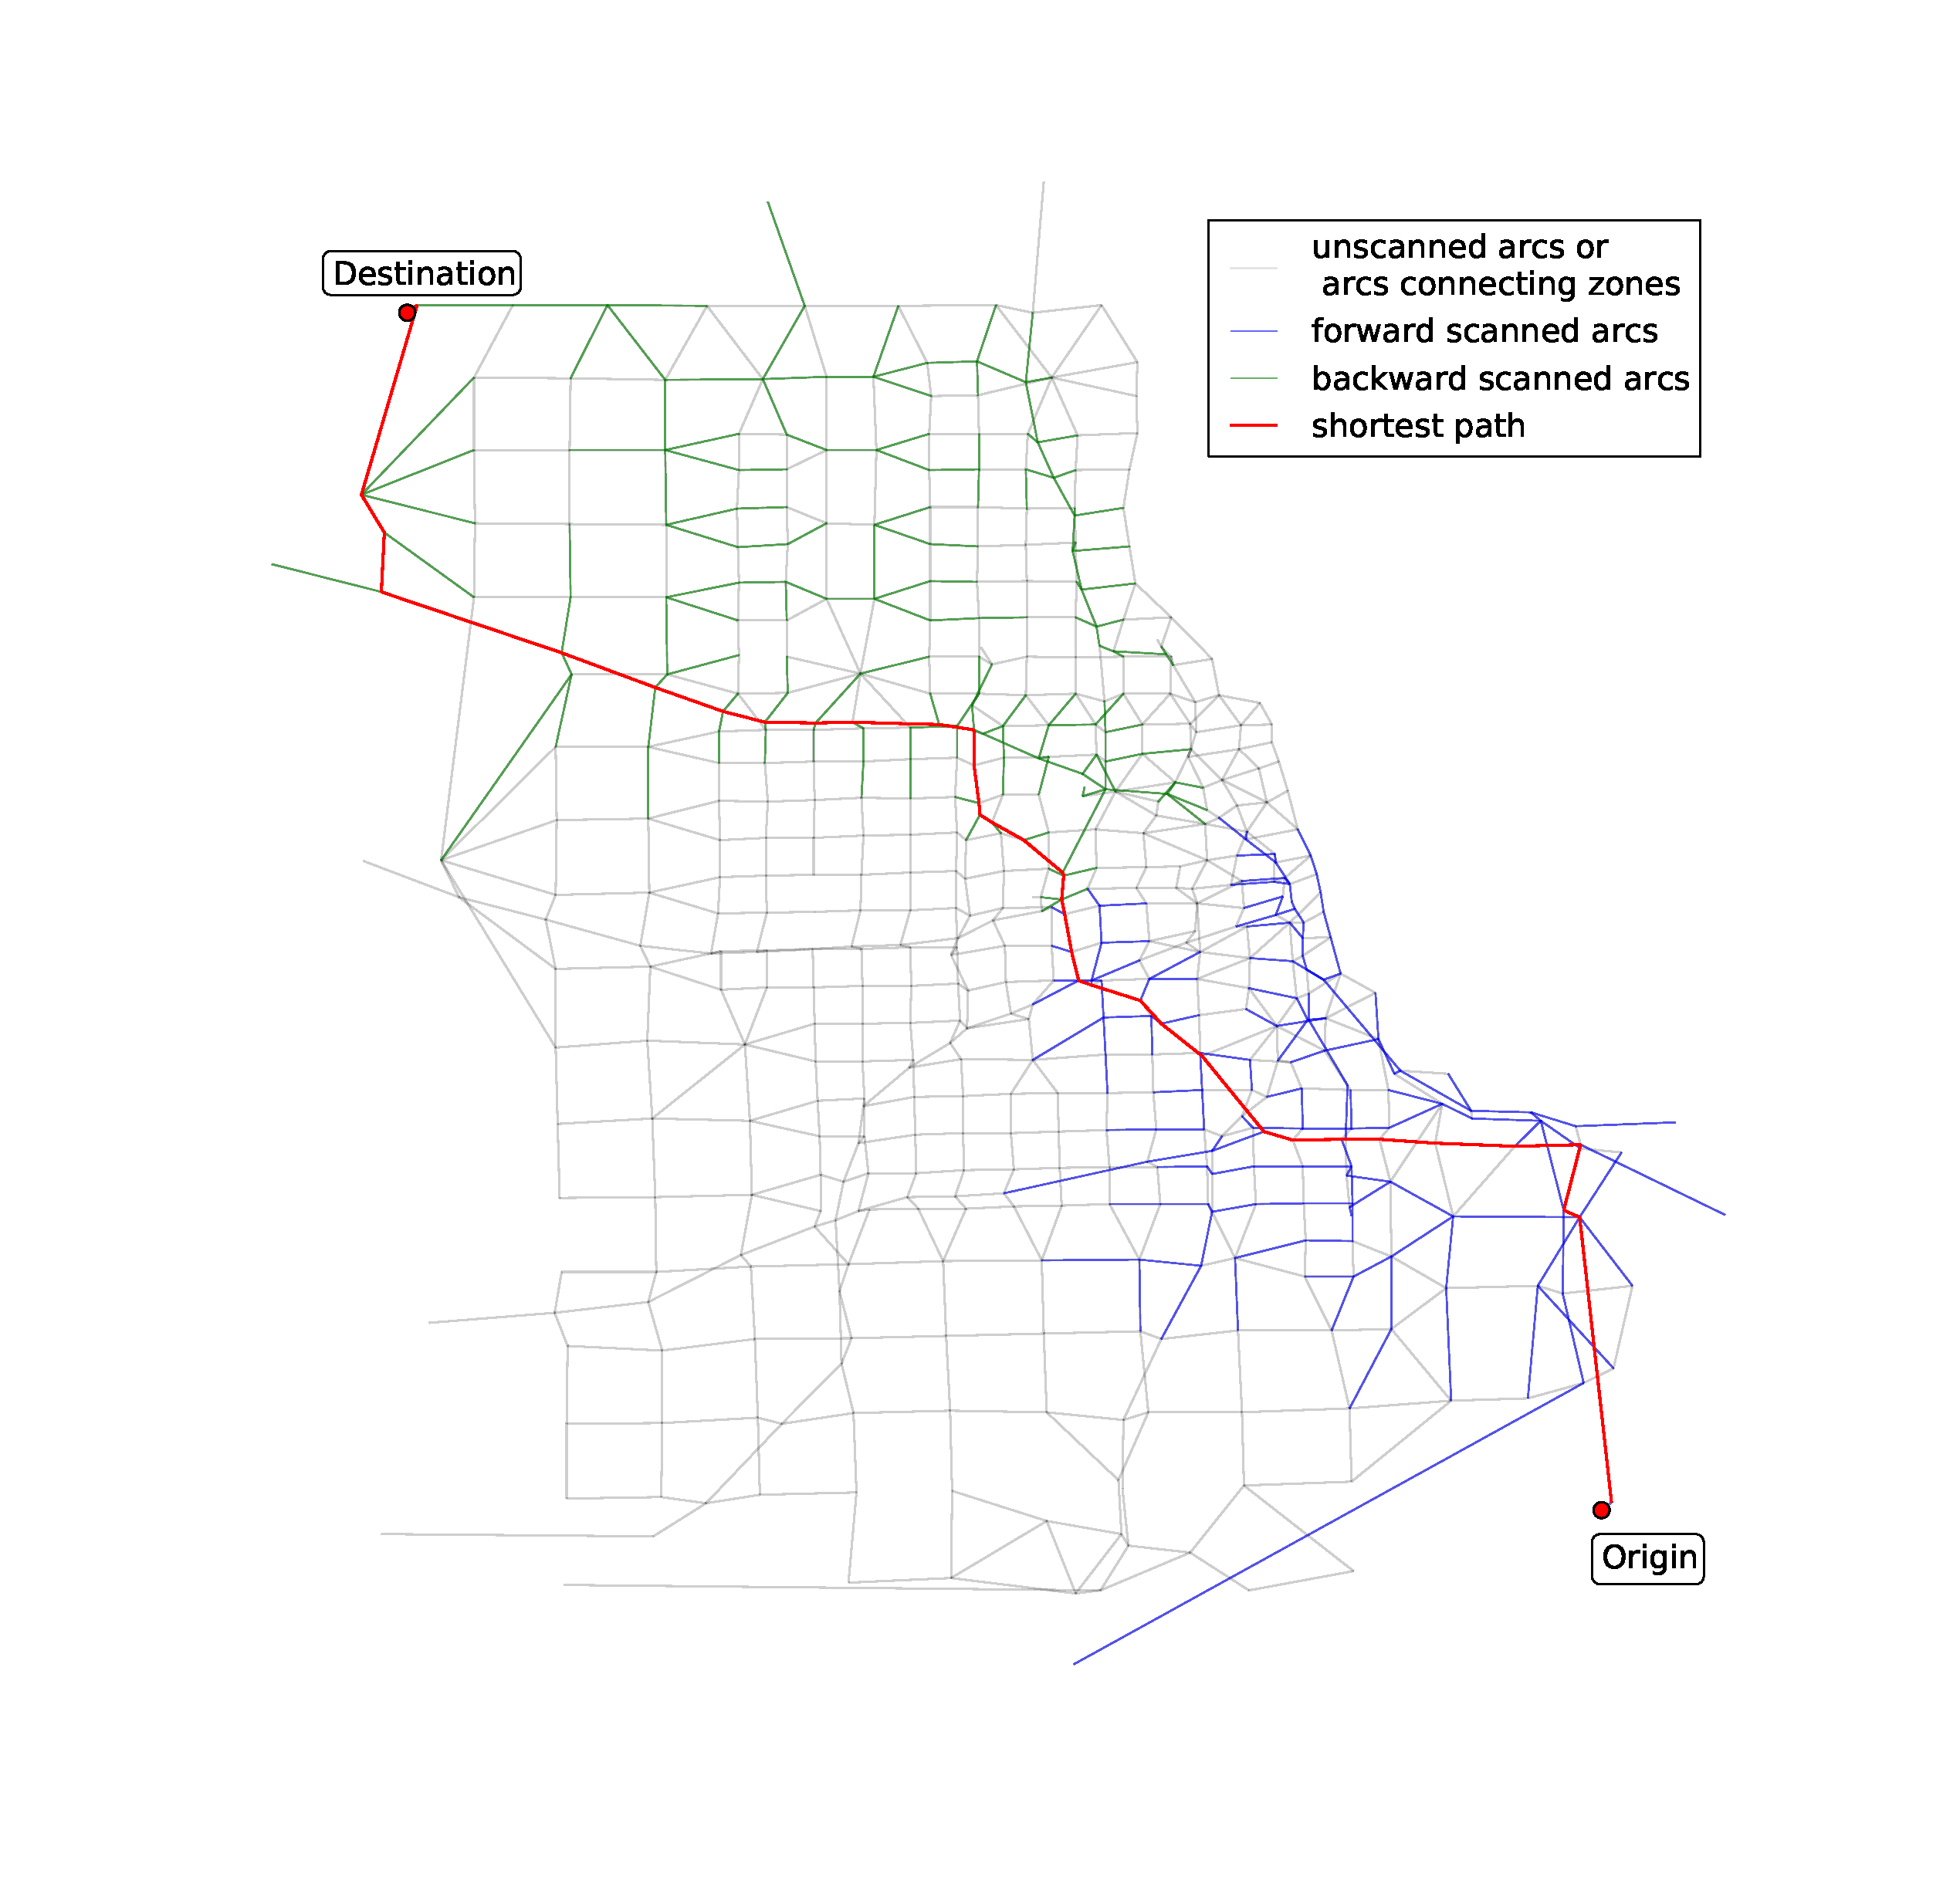
\includegraphics[width=\paperwidth, height=\paperheight, keepaspectratio,trim=0 120px 48px 120px,clip]{img/chicago_astar_bidirect}
    \end{center}
\end{frame}

\begin{frame}{A* Search vs Bidirectional A* Search}
    \makebox[\linewidth]{
        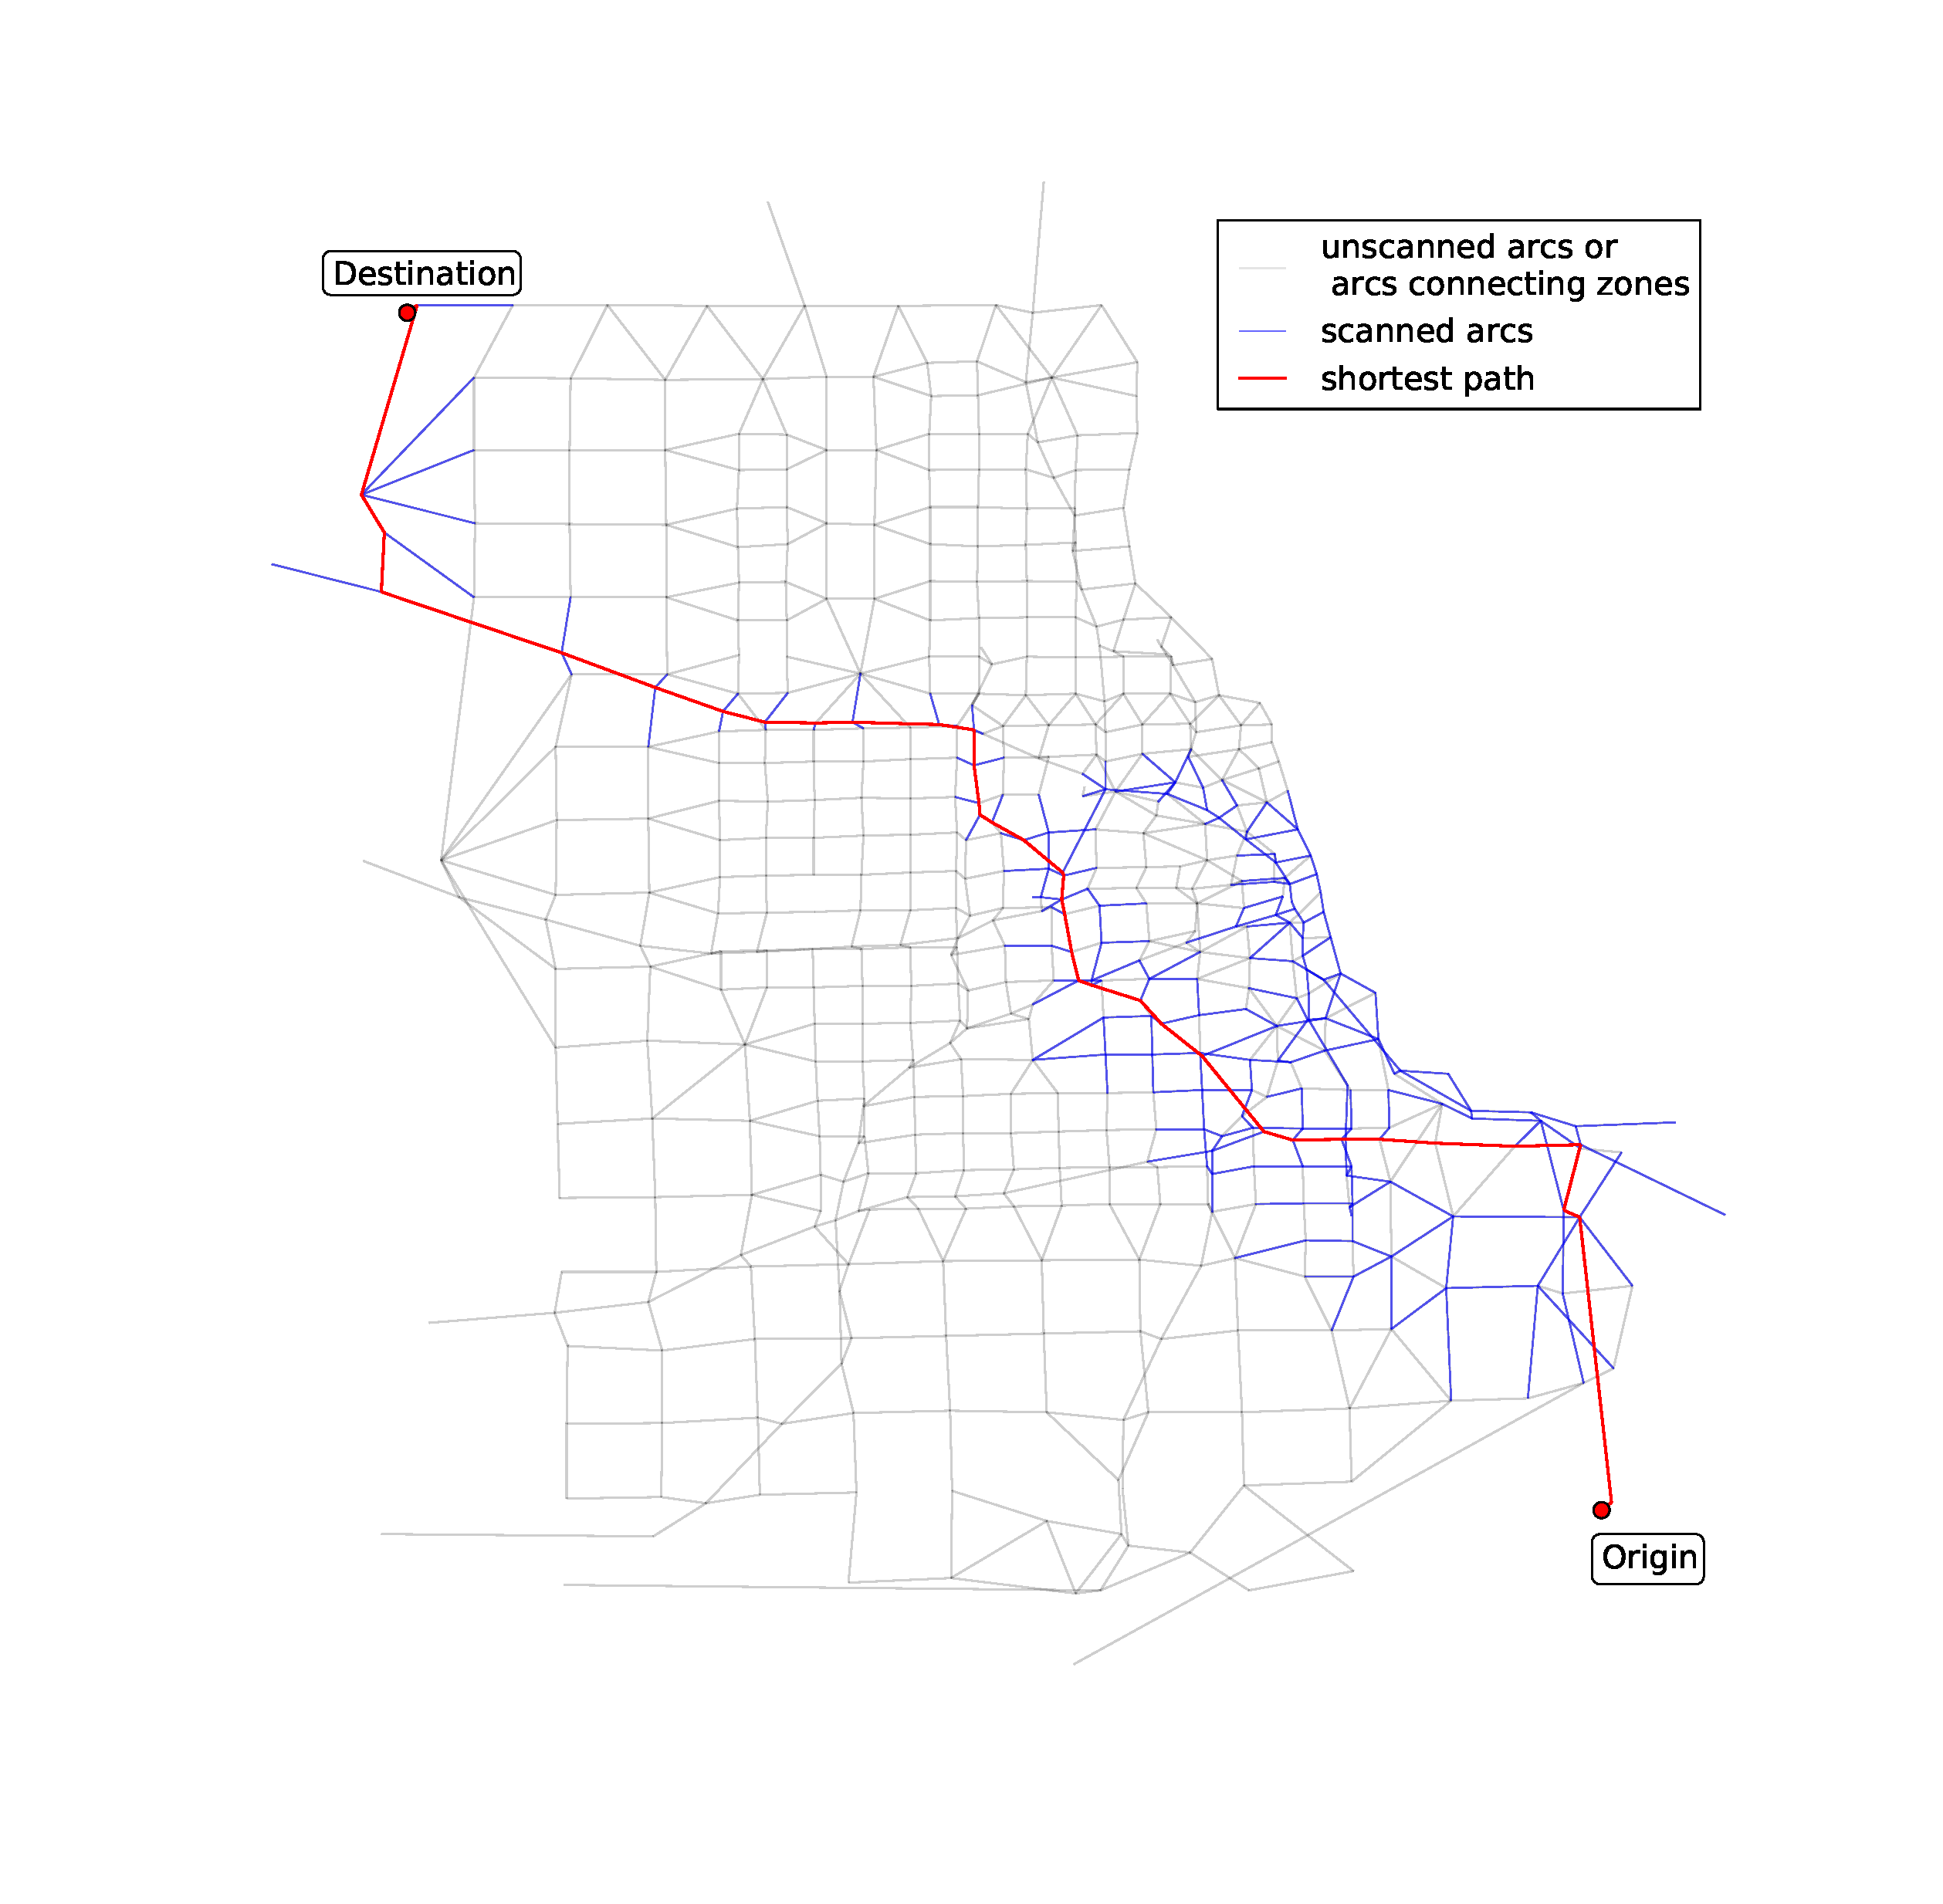
\includegraphics[width=0.5\paperwidth,height=\paperheight,trim=0 0 48px 120px,clip]{img/chicago_astar}
        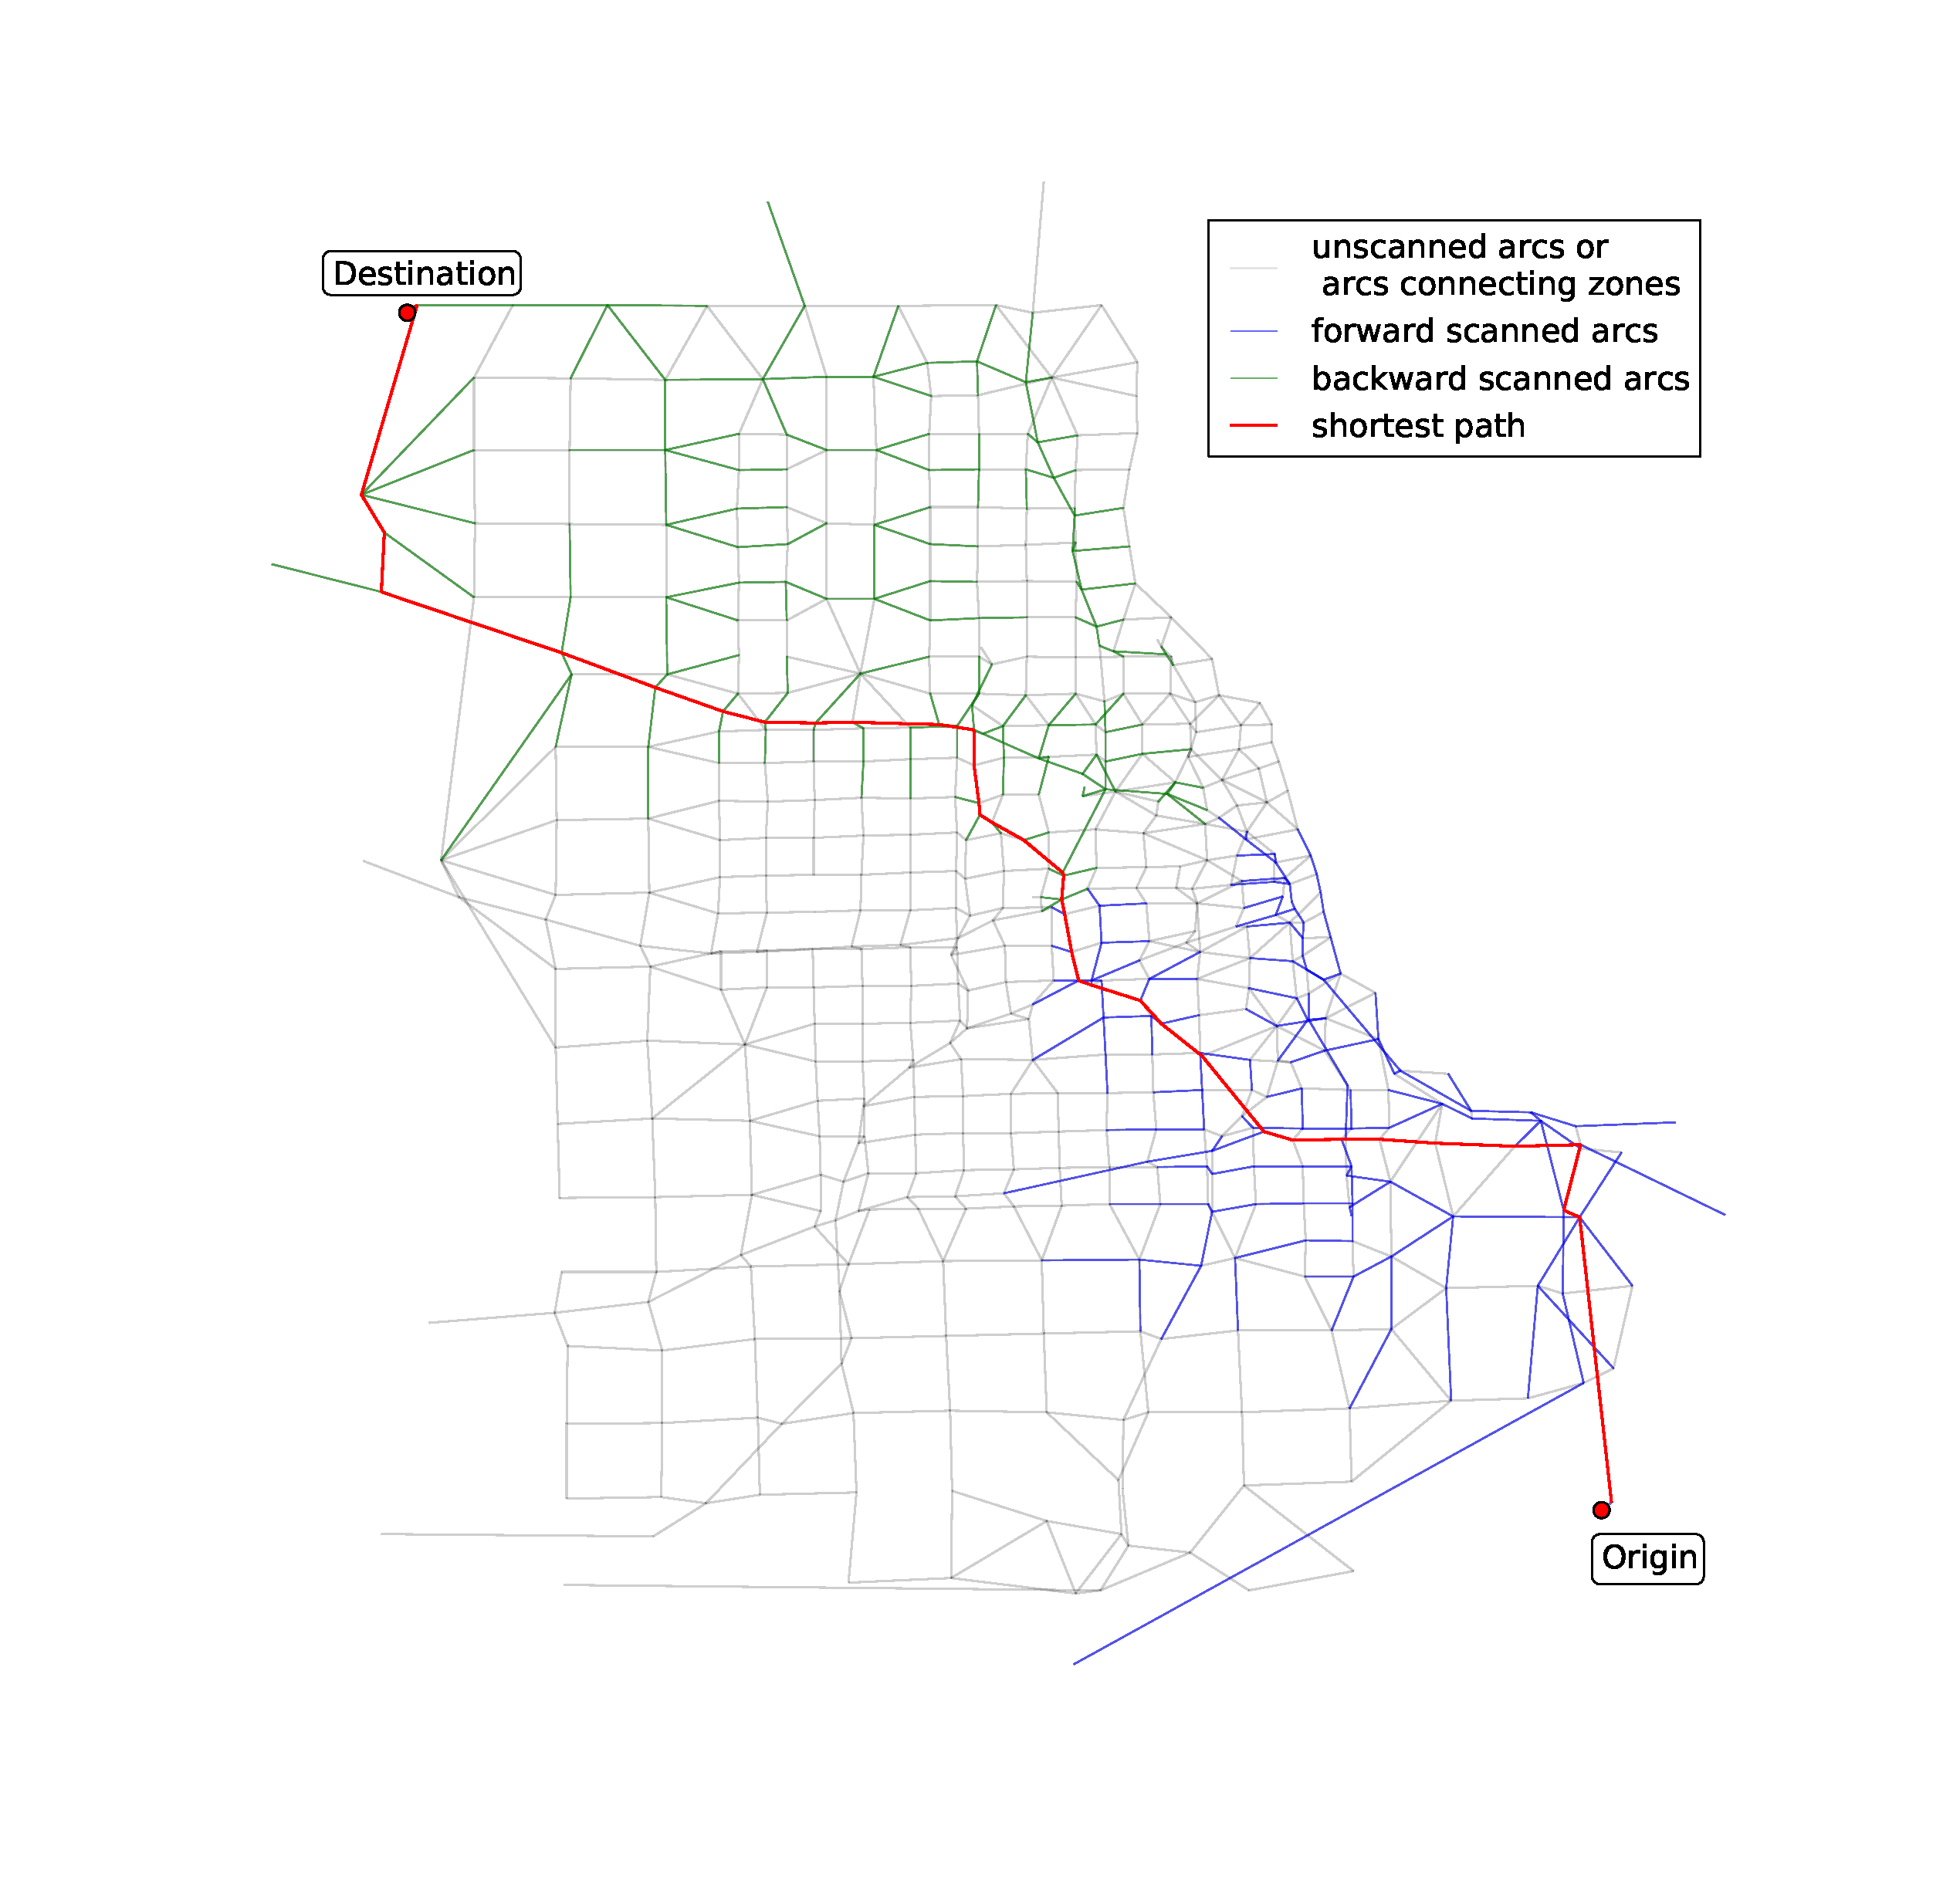
\includegraphics[width=0.5\paperwidth,height=\paperheight,trim=0 0 48px 120px,clip]{img/chicago_astar_bidirect}
    }
\end{frame}

\section{Results - speed ups}
\begin{frame}
    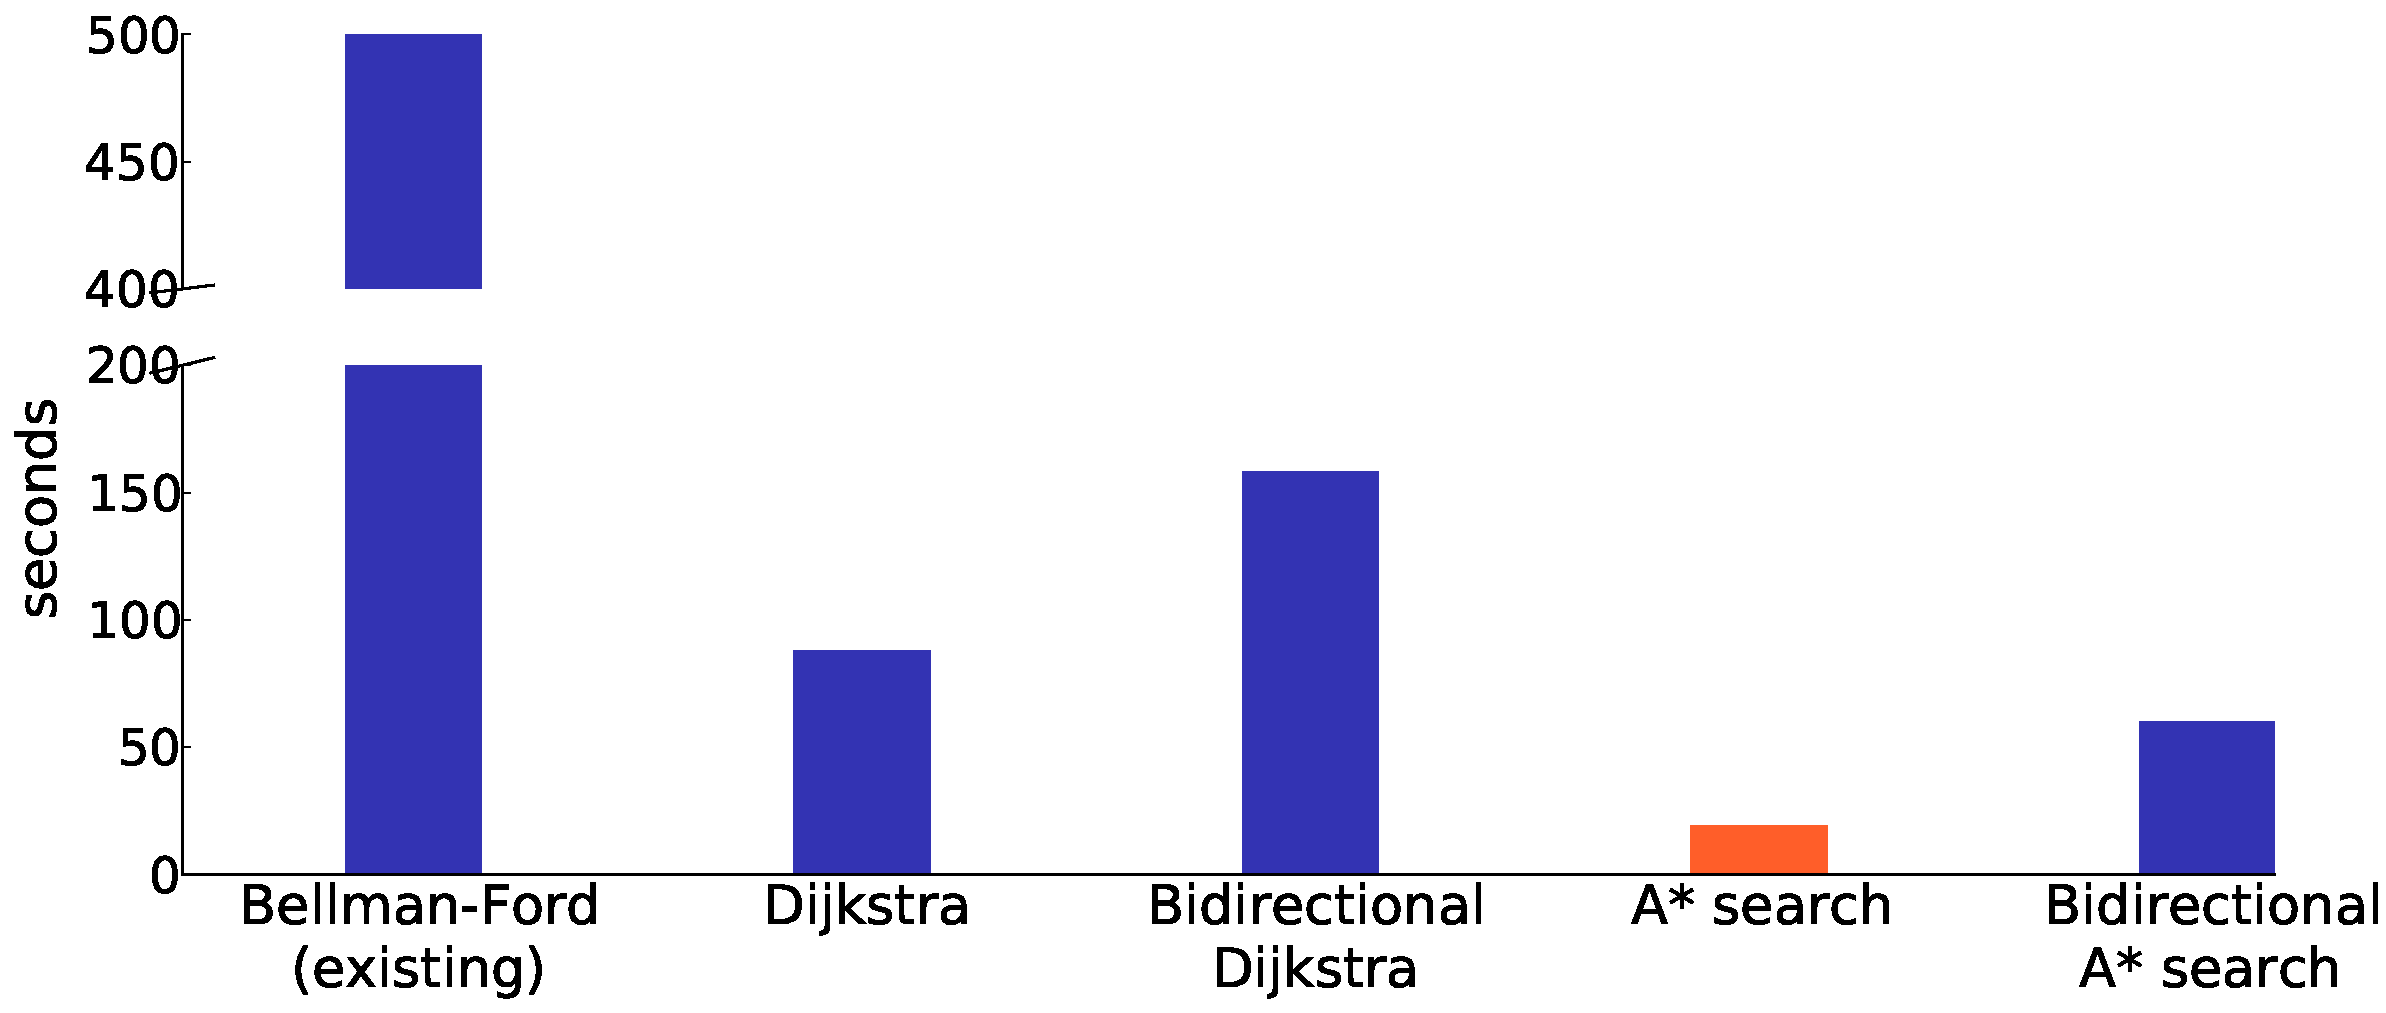
\includegraphics[width=\paperwidth, height=\paperheight, keepaspectratio, trim=0 0 0 120pt, clip]{img/runtime}

    \tikzstyle{block} = [circle, draw, inner sep=0pt,minimum size=1pt]
    \begin{tikzpicture}[overlay, shift={(1.6,-0.2)}]
        \node [block, minimum size= 1.4pt] (a) {};
        \node [block, minimum size= 7.9pt] (b) [xshift=1cm, right of=a] {};
        \node [block, minimum size= 4.3pt] (c) [xshift=0cm, right of=b] {};
        \node [block, minimum size= 93pt] (d) [xshift=6cm, right of=c] {};

        \node [above] at (a.north) {\tiny 10 iters};
        \node [above] at (b.north) {\tiny 27 iters};
        \node [above] at (c.north) {\tiny 126 iters};
        \node [above] at (d) {\tiny 25 iters};
    \end{tikzpicture}
\end{frame}

\end{document}
